%================================================================
\chapter{Results and Discussion}\label{chap:results_discussion}
%================================================================
In this chapter, we will investigate and characterize models discussed in earlier chapters. We will also detail how the various models are configured, and how numerical methods are used for characterization. The results will be briefly commented on as they are presented, with a more in-depth discussion at the end of each section.

%In \cref{sec:Vanishing Gradient Phenomenon}, we investigate and compare the vanishing gradient phenomenon for QNNs, QCNs and DNNs by studying how the magnitudes of their gradients vary as a function of architecture. The behaviour with respect to the number of layers is emphasized.

%In \cref{sec:Investigating the Loss Landscape}, we characterize the geometry of the loss landscape of QNNs, QCNs and DNNs by studying their EFIM spectra, as presented in \cref{sec:EFIM}. The result will be used to asses the trainability of different models and predict how architecture affects training.

%In \cref{sec:Expressivity}, we assess the expressivity of QCNs and compare them to DNNs using trajectory length as presented in \cref{sec:TrajectoryLength}. This is done for both trained and untrained models.

%In \cref{sec:Training Models}, we test models in a practical setting, and give support to previous results and analyses in this thesis by fitting them to mixed Gaussian data in multiple dimensions. This is done both using idealised simulation(see \cref{sec:Exact Expectation Value}), and simulated, noisy hardware.


%================================================================
\section{Vanishing Gradient Phenomenon}\label{sec:Vanishing Gradient Phenomenon}
%================================================================
In this section, we investigate and compare the vanishing gradient phenomenon for QNNs, QCNs and DNNs by studying how the magnitudes of their gradients vary as a function of architecture. First, we study how the gradients of QNNs behave as the number of qubits and repetition of the ansatz increase. Then, the local gradients \cref{eq:localGradients} of QCNs are studied for different number of qubits, nodes and layers. Lastly, the vanishing of the total gradient \cref{eq:derivweightsQCN} is investigated.


%================================================================
\subsection{Vanishing Gradient in QNNs}\label{sec:Vanishing Gradient for QNNs}
%================================================================
We start by investigating the magnitude of the gradient of QNNs for different number of qubits and repetitions of the ansatz. We use qubit encoding \cref{fig:qubitencoding} with $R_y$ rotations for feature encoding, and the simple ansatz \cref{eq:simple ansatz} for processing. This combination was chosen as it was found to yield the largest gradient. To derive an output, we calculate the expected parity \cref{eq:parity} using ideal simulation, as explained in \cref{sec:Exact Expectation Value}. We calculate the average magnitude of the gradient using \cref{eq:magnitude QNN}, with $T=10$ different realizations of the parameters to increase the statistical significance of the result. To get a representative result for a large feature space, we sample features $\mathcal{X} = \{\boldsymbol{x}^{(1)}, \cdots, \boldsymbol{x}^{(N)}\}$ uniformly as $\mathcal{X} \sim U(-\frac{\pi}{2}, \frac{\pi}{2})^{[N,p]}$. We use $N=100$ samples, and the number of features $p$ is set equal to the number of qubits for each QNN. The QNNs are also initialized in the standard way, i.e. sampling parameters as $\theta_j \sim U(-\pi, \pi)$. The resulting magnitude of the gradients for different number of qubits and ansatz repetitions can be seen in figure \cref{fig:QNN_vanishing}.

\begin{figure}[H]
    \centering
    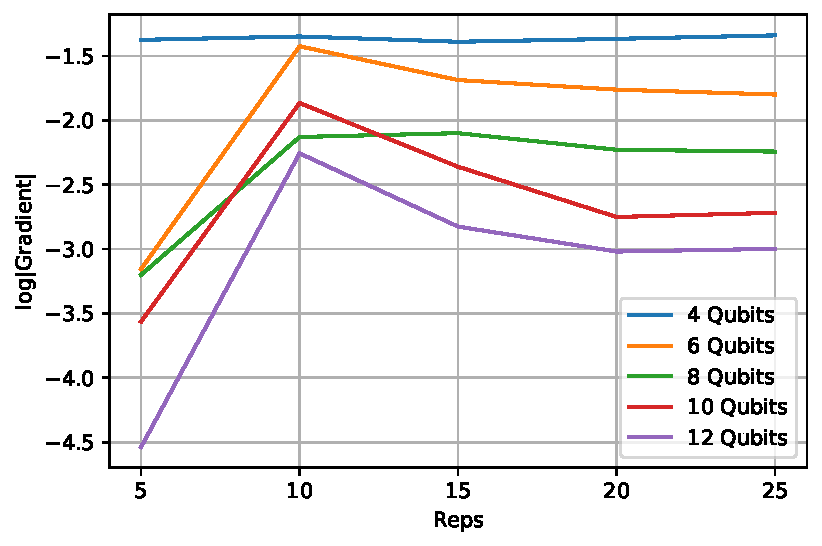
\includegraphics[width=12cm]{latex/figures/vanishing_gradient_QNN.pdf}
    \caption{Average magnitude of gradients for QNNs with different numbers of ansatz repetitions and qubits. The QNNs utilize qubit encoding with $R_y$ rotations, the simple ansatz for processing, and parity sampling to derive an output. The QNNs are fed $N=100$ points of uniformly sampled points, where the number of features is set equal to the number of qubits.}
    \label{fig:QNN_vanishing}
\end{figure}

From the above figure, we see that our implementation of QNNs results in a gradient that vanishes in the exponential regime with respect to the number of qubits. Also, the vanishing is stronger for a higher number of repetitions of the ansatz. This behavior can be explained by the fact that QNNs are a special variant of PQCs. By encoding random inputs and randomly initializing the parameters, the QNN essentially approaches a random circuit as they grow deeper. As shown by \citet{McClean_2018}, and discussed in \cref{sec:BarrenPlateus}, randomly initialized PQCs tend to produce gradients closely centered around zero as the number of qubits are increased, which also applies for our implementation of QNNs.  

%================================================================
\subsection{Vanishing Local Gradient in QCNs}\label{sec:Vanishing Local Gradients in QCNs}
%================================================================

An interesting feature of QCNs is the ability to create larger models by introducing more circuits, rather than wider and deeper ones. As the gradients of QNNs tend to vanish with higher numbers of qubits, we want to investigate how the gradients of smaller QNNs behave when they enter as nodes in a QCN architecture.

The QNNs used as nodes to construct QCNs here are set up and initialized in the manner explained in \cref{sec:Vanishing Gradient for QNNs}, but always with two repetitions of the simple ansatz to keep each circuit shallow. Also, we sample input data uniformly as $\mathcal{X} \sim U(-\frac{\pi}{2}, \frac{\pi}{2})^{[N,p]}$, with $N=100$ and the number of features $p$ set to the number of qubits used in the each node. In this section, all QCNs have 8 layers with $d$ number of nodes each, where $d$ range from four to eight. The number of qubits in each node will also be set to $d$. Further, the outputs of each hidden layer is scaled to the interval $[-\pi, \pi]$ to make full use of the qubit encoding in the subsequent layer, as explained in \cref{sec:Configuring QCNs and DNNs}.

In order to investigate the average behavior of the local gradients \cref{eq:localGradients} for each layer, we calculate their magnitude averaged over each layer, the samples and $T = 10$ different realizations. This quantity is given by \cref{eq:magnitude local}, and is plotted in \cref{fig:QCN_local_vanishing} for various layers of different QCNs. In addition, the standard deviation of this quantity is estimated over the different realizations, serving as a confidence interval seen in the figure. 

\begin{figure}[H]
    \centering
    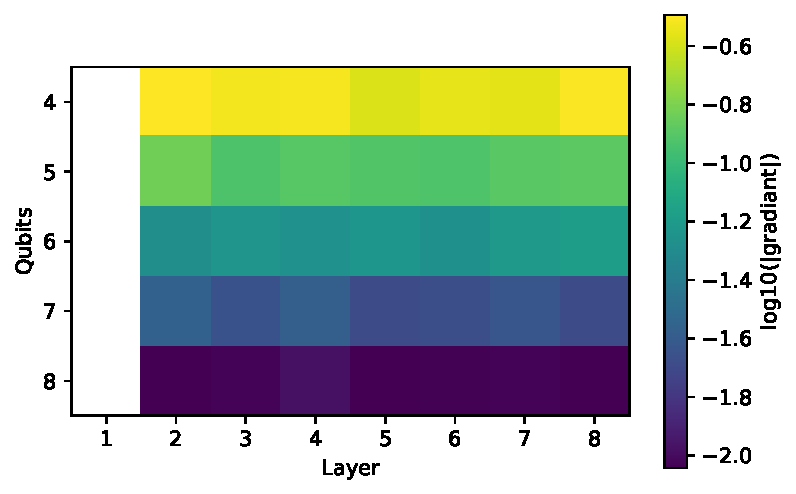
\includegraphics[width=12cm]{latex/figures/vanishing_gradient_partial_input.pdf}
    \caption{Average magnitude of local gradients \cref{eq:localGradients} calculated for each layer for various QCNs with eight layers. This quantity was calculated using \cref{eq:magnitude local}. The number of qubits per node is constant for each QCN, and the number of nodes per layer is set equal the number of qubits. The QCNs are fed $N=100$ points of uniformly sampled points, where the number of features is set equal the number of qubits. The standard deviation is calculated over ten different realizations of the model parameters.}
    \label{fig:QCN_local_vanishing}
\end{figure}

In the above figure we see the average magnitude of the local gradients for different layers and number of qubits. The local gradients of the QCNs tend to vanish exponentially in the number of qubits, similar to the gradients of single-circuit QNNs seen in \cref{fig:QNN_vanishing}. However, the relative position along the depth of the QCN does not seem to affect the magnitude. This can be seen from the overlapping confidence intervals of the magnitudes for each number of qubits. Any variation of the average magnitude between the layers is thus likely just noise induced by the low number of ten parameter realizations, and does not indicate significant differences.

%================================================================
\subsection{Vanishing Total Gradient in QCNs}\label{sec:Vanishing Total Gradients in QCNs}
%================================================================

%In the previous section, it was shown that scaling up QCNs by adding more layers did not effect the number of shots needed to sufficiently estimate the local gradients of each QNN. This is in opposition to single-QNN models, whose gradient vanishes as both the number of qubits and repetitions are increase, as seen in \cref{fig:QNN_vanishing}.

In the previous subsection, we showed that the magnitude of local gradients of any layer is independent of the relative position of that layer in the QCN model. However, the parameters of are not updated using the local gradients directly. Rather, they are updated using the total gradient \cref{eq:derivweightsQCN}, which is calculated by combining the local gradients using back propagation \cref{eq:errorQCN}. We need to investigate how the magnitude of the total gradient \cref{eq:derivweightsQCN} behaves as a function of layers and qubits. 

In this section, the total gradient is calculated using the local gradients from the numerical experiments in \cref{sec:Vanishing Local Gradients in QCNs}. As previously, the magnitude of the total gradient is averaged over each layer, the samples and ten realizations of the parameters using \cref{eq:magnitude QCN DNN}. This quantity is plotted in \cref{fig:QNC_vanishing_total} for different layers and number of qubits. For comparison, it also shows the magnitude of the total gradient of two DNNs with the same number of layers and similar number of parameters as the four and eight-qubit QCN.

\begin{figure}[H]
    \centering
    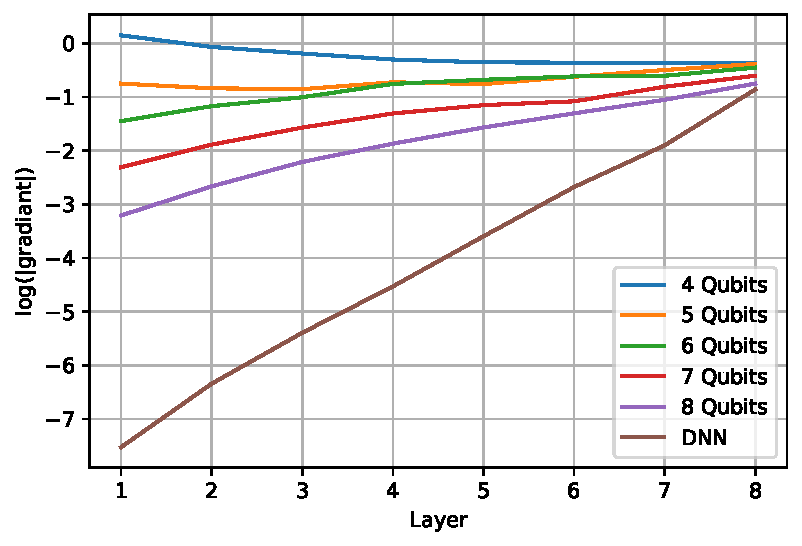
\includegraphics[width=12cm]{latex/figures/vanishing_gradient_total.pdf}
    \caption{Average magnitude of the total gradient \cref{eq:derivweightsQCN} calculated for each layer for various 8 layer QCNs. This quantity is calculated using \cref{eq:magnitude QCN DNN}. The number of qubits per node are constant for each QCN, and the number of nodes per layer is set equal the number of qubits.  For comparison, the same quantity is also calculated for two DNNs with 5 and 11 nodes, respectively. The DNNs have tanh activations on all layers.}
    \label{fig:QNC_vanishing_total}
\end{figure}

From \cref{fig:QNC_vanishing_total}, we see that the total gradient for a given layer in the DNN tends to vanish exponentially in the number of layers after it. This is a well-known phenomenon for classical neural networks, often explained by the saturation of the activation function during feed forward \cite{shalevshwartz2017failures}. (Write about this under neural network theory).

As with the DNN, the QCNs also exhibit a vanishing total gradient with increasing number of layers, with a strong dependence on the number of qubits in each node. As we see in \cref{fig:QCN_local_vanishing}, the total gradient vanishes faster for higher number of qubits in each node. This phenomenon can be related to the magnitude of the local gradients. As the error \cref{eq:lastLayerErrorQCN} of the QCN is propagated backwards using \cref{eq:errorQCN}, it accumulates the local gradients $\frac{\partial \boldsymbol{a}^{l+1}_k}{\partial \boldsymbol{a}^{l}_j}$ as factors. As the number of qubits increases, the local gradients tend to decrease. Accumulating small factors will cause the error to decrease faster, exponentially so for each layer. However, if these factors are large, the error tends to decrease more slowly, and hence also the total gradient. This is the case for architectures with few qubits per node, as discussed in \cref{sec:Vanishing Local Gradients in QCNs}.

%================================================================
\subsection{Discussion}\label{sec:Vanishing Gradient Phenomenon Discussion}
%================================================================
The results of \cref{sec:Vanishing Gradient for QNNs} show that increasing the model size of QNNs by adding more qubits and repetitions of the ansatz results in an exponential decay of their gradients. As explained in \cref{sec:BarrenPlateus}, this means that exponentially many shots are required in order to obtain a good signal-to-noise when estimating the gradient. If the gradient is too noisy, optimization using gradient descent and similar methods may essentially result in a random walk in parameter space that fails to converge \cite{skolik2020layerwise}. This becomes even more problematic in the presence of noise introduced by real hardware, as discussed in \cref{sec:Noisy Simulation}. Ultimately, this indicate that the training of QNNs can become intractable as they are increased in size to solve harder learning problems.    

In \cref{sec:Vanishing Local Gradients in QCNs}, we see that the local gradients of QCNs also vanish exponentially fast in the number of qubits, but are independent of the overall number of layers. In other words, the local gradients of any layer are unaffected by outputs produced by the previous layer. This suggests that QCNs can be scaled up by making them deeper, without affecting the magnitude of the local gradients. Consequently, a constant number of shots can be used for each node during estimation to obtain a certain signal-to-noise ratio, making their estimations tractable on a quantum computer. 

Even though the magnitude of local gradients of QCNs tends to stay constant in the number of layers, we see in \cref{sec:Vanishing Total Gradients in QCNs} that back propagation still induces an exponentially vanishing total gradient for sufficiently many qubits. This is due to the accumulation of small factors when the local gradients are combined using backpropagation. This behavior is similar to that of DNNs, with the gradient vanishing faster for initial layers. However, the vanishing was not as severe for a conservative number of qubits. For 4 qubits, the gradient actually tended to increase. For 8 qubits, and presumably above, the gradient vanished faster for QCNs than for similarly sized DNNs.  

An interesting observation is that the vanishment caused by back propagation happens in a purely classical part of the optimization, with the local gradients stored as floating-point numbers. This means that even though the total gradient tends to decrease exponentially with the number of layers, it does not introduce an exponential overhead on the quantum computer by requiring more shots. However, the overhead increases exponentially for single-QNN models as discussed in \cref{sec:BarrenPlateus}. Put another way, QCNs' use of several smaller circuits, rather than one large, moves the estimation of vanishing quantities (e.g. the gradient) from quantum expectation values to classical computation. 



%================================================================
\section{Investigating the Loss Landscape}\label{sec:Investigating the Loss Landscape}
%================================================================
We explore the geometry of the loss landscape of randomly initialized QNNs, QCNs and DNNs, and quantify their degree of distortion and flatness by studying the eigenvalue spectrum of the EFIM \cref{eq:EmpiricalFisher}. Looking at \cref{eq:EmpiricalFisher}, we see that the EFIM, unlike the Hessian, is independent of targets $y^{(i)}$. This makes the analysis data agnostic. The input data sampled uniformly as $\mathcal{X} \sim U(-\frac{\pi}{2}, \frac{\pi}{2})^{[N,p]}$, like earlier. For the DNNs, the features are standardized as explained in \cref{sec:Scaling Features}. Here, we use $N=200$ samples and either $p=4$ or $p=6$ inputs, depending on the model. For each model, the EFIM is calculated ten times for different realizations of the model parameters. The resulting spectrum is then averaged over different realizations to produce a more statistically significant result. For a complete description of the models analyzed in this section, see \cref{tab:FIM models}.

\begin{table}[H]
\caption{Description of the architecture of the models analyzed in this section. \emph{Reps} is the number of ansatz repetitions, and $n_{\theta}$ is the number of model parameters. The QNN and QCN models use ideal simulation to derive outputs. The DNN models use tanh activation in all layers. The parameters of the models are appropriately initialized as described in \cref{sec:Initialization}.} 
\centering
\begin{tabular}{|l|l|l|l|l|l|l|l|}
\hline
Model &Type & Qubits& Reps & Layers & Nodes & Encoder        & $n_{\theta}$ \\ \hline
A    & QNN & 4& 18   & 1      & 4     & RZZ Encoding   & 72  \\ \hline
B    & QCN & 4& 3    & 2      & 4     & Qubit Encoding & 60 \\ \hline
C    & QCN & 4& 2    & 3      & 4     & Qubit Encoding & 72  \\ \hline
D    & QCN & 4& 1    & 5      & 4     & Qubit Encoding & 68  \\ \hline
E    & DNN & NA& NA   & 3      & 6     & NA             & 79 \\ \hline
F    & QNN & 6& 26   & 1      & 6     & RZZ Encoding   & 156  \\ \hline
G    & QCN & 6& 4    & 2      & 6     & Qubit Encoding & 168 \\ \hline
H    & QCN & 6& 2    & 3      & 6     & Qubit Encoding & 156  \\ \hline
I    & QCN & 6& 1    & 5      & 6     & Qubit Encoding & 150  \\ \hline
J    & DNN & NA& NA   & 3      & 9     & NA             & 163 \\ \hline
\end{tabular}
\label{tab:FIM models}
\end{table}

\cref{fig:FIM Comparison} compares the EFIM spectra of QNNs, QCNs and DNNs. Their architectures are chosen so that the models have approximately equal numbers of parameters. This is to ensure a fair comparison. 

\begin{figure}[H]
    \centering
    \begin{subfigure}[t]{0.5\textwidth}
        \centering
        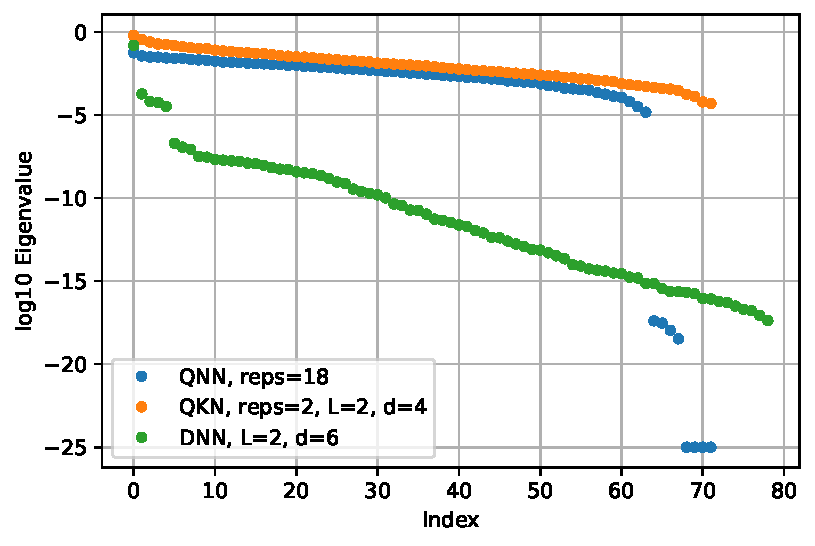
\includegraphics[height=1.9in]{latex/figures/FIM_qubits_4.pdf}
        \caption{QNN and QCN with four qubits in each circuit.}
    \end{subfigure}%
    ~ 
    \begin{subfigure}[t]{0.5\textwidth}
        \centering
        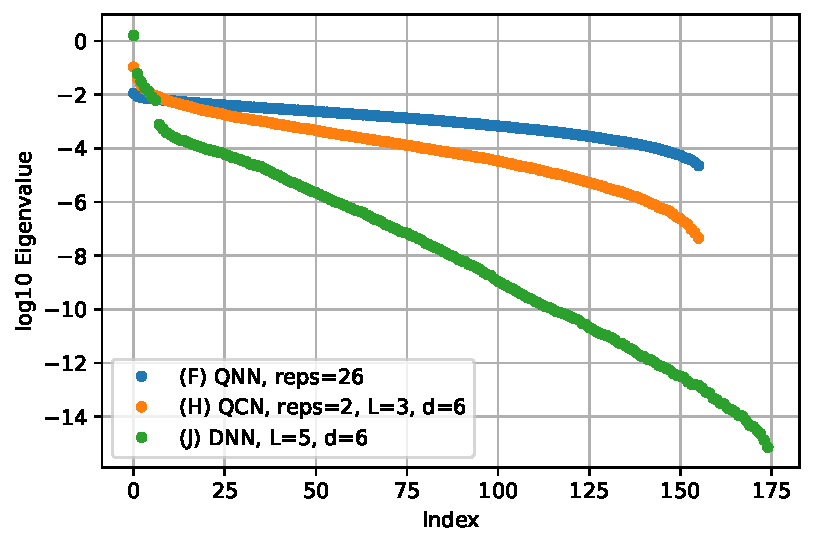
\includegraphics[height=1.9in]{latex/figures/FIM_qubits_6.pdf}
        \caption{QNN and QCN with six qubits in each circuit.}
    \end{subfigure}
    \caption{Comparison of EFIM spectrum between QNNs, QCNs and DNNs, calculated for uniform data. For details about the architectures, see \cref{tab:FIM models}. \emph{reps} is the number of ansatz repetitions, \emph{L} is the number of layers, and \emph{d} is the number of nodes.}
    \label{fig:FIM Comparison}
\end{figure}

Looking at the spectra of the DNNs in \cref{fig:FIM Comparison}, we see the characteristic result of a singular large eigenvalue, with the rest sitting close to zero. This indicates that DNN models exhibit a loss landscape that is very flat in all but one direction where it is extremely distorted. We also see that the spectra of our implementation of QNNs are much more uniformly distributed compared to the DNN models. This results in a loss landscape that is significantly distorted in most directions, rather than just one. 

Moving over to the QCNs, we see from \cref{fig:FIM Comparison} that the spectra of the three layer QCNs exhibit much the same uniformity as the QNNs. A more thorough comparison between different QCNs is shown \cref{fig:FIM QCN}. In this figure, we vary the number of layers of the QNCs and the number of repetitions (i.e. the number of times the ansatz is repeated for each node), while keeping the total number of parameters roughly constant. In doing this, we get to precisely shift how much of the complexity of a given QCN results from the complexity of each node or the overall structure of the network.

\begin{figure}[H]
    \centering
    \begin{subfigure}[t]{0.45\textwidth}
        \centering
        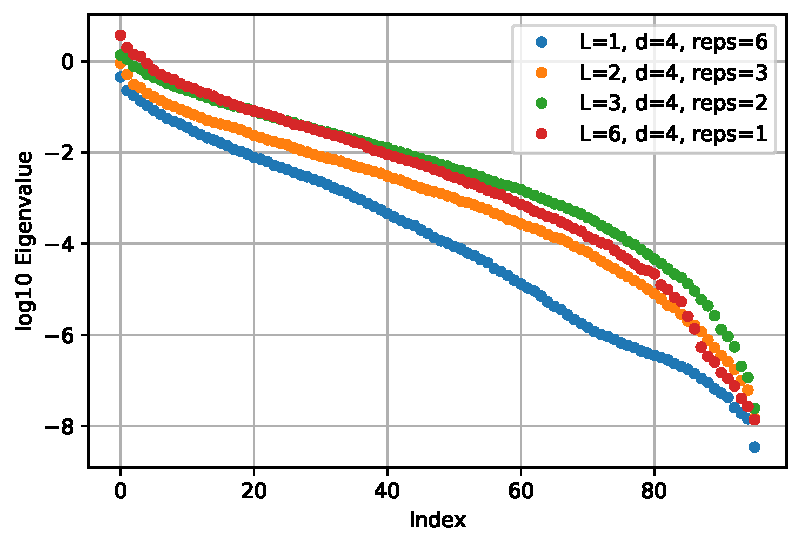
\includegraphics[height=1.8in]{latex/figures/FIM_qubits_4_comparison.pdf}
        \caption{Comparison of the EFIM spectra for different QNNs and QCNs with four qubits.}
        \label{fig:FIM QCN a}
    \end{subfigure}%
    ~ 
    \begin{subfigure}[t]{0.45\textwidth}
        \centering
        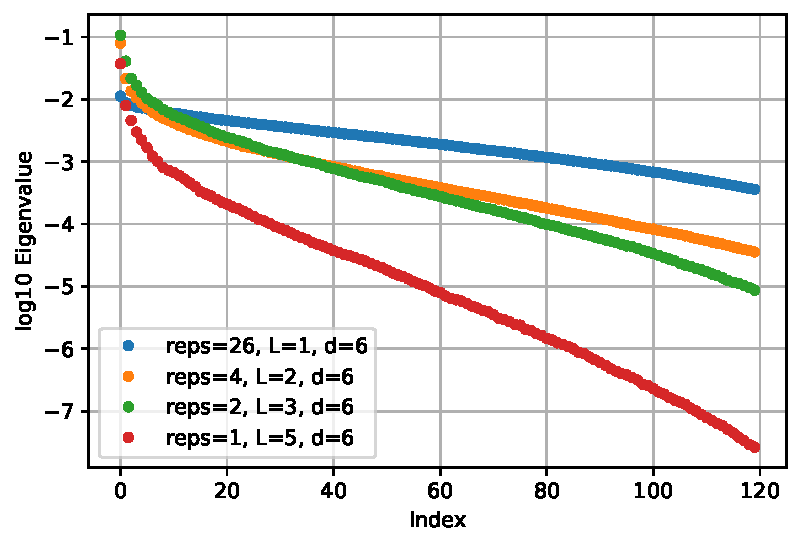
\includegraphics[height=1.8in]{latex/figures/FIM_qubits_6_comparison.pdf}
        \caption{Comparison of the EFIM spectra for different QNNs and QCNs with six qubits.}
        \label{fig:FIM QCN b}
    \end{subfigure}
    \caption{Comparison of the EFIM eigenvalue spectrum between different QNNs and QCNs, calculated for uniform data. For details about the architectures, see \cref{tab:FIM models}. \emph{reps} is the number of ansatz repetitions, \emph{L} is the number of layers, and \emph{d} is the number of nodes.}
    \label{fig:FIM QCN}
\end{figure}

\cref{fig:FIM QCN a} shows that, for four qubits, the spectra of the different QCNs exhibit roughly the same uniformity as the QNN, with the eigenvalues staying within roughly an order of magnitude of each other. Going up to six qubits, \cref{fig:FIM QCN b} shows that the spectrum tends to concentrate more around zero for increasing number of layers. This is likely related to the vanishing of the gradient induced by back propagation. For four qubits, this is not as big of a problem since the local gradients are relatively big and hence the total gradient. However, for six qubits, the local gradients tend to vanish. This results in the gradient vanishing faster when increasing the number of layers, which in turn results in a flatter landscape. 


%================================================================
\subsection{Discussion}\label{sec:Loss Landscape Discussion}
%================================================================
The highly uneven EFIM spectrum of DNNs indicates a loss landscape that is strongly distorted in one direction and mostly flat otherwise. This result is consistent with the findings of \citet{karakida2019universal} and \citet{abbas2020power}. The former authors point out that strong distortions in some directions indicate that the model outputs are highly sensitive to changes in parameter space in exactly these directions, and likewise not sensitive to changes in the others. This tend to slow training when using gradient descent and similar methods, as too high learning rate leads to overstepping in the distorted directions, while a low learning rate changes the model insignificantly in the flat directions. 

For the QNNs, we found the EFIM spectrum to be much more uniform than that of a comparable DNN. \citet{abbas2020power} came to the same conclusion for their QNN models, and argued that this uniformity of the spectrum meant that the landscape was more well-condition for optimization, and thus should train faster. They strengthened this hypothesis by showing experimentally that their QNNs reduced loss faster than DNNs for equal numbers of epochs. 

We found that QCNs with four qubits exhibit similar uniformity of the EFIM spectrum as QNNs. For six qubits, the spectrum became increasingly more skewed, with a worsening effect for more layers. However, they still showed several order of magnitude larger eigenvalues that DNNs, suggesting that small-scale QCNs should train comparably faster than DNNs, like QNNs.

%================================================================
\section{Expressivity}\label{sec:Expressivity}
%================================================================
We investigate the expressivity of QCNs and DNNs using the trajectory length method of \citet{raghu2017expressive}, as described in \cref{sec:TrajectoryLength}. The trajectory length will first be  studied for randomly initialized QCNs for varying number of qubits in each node. Then, for some selected QCNs, the trajectory length will be investigated as the models are gradually fitted on 2D mixed Gaussian data. The results in both cases will be compared to similar DNNs, with approximately the same number of parameters for fair comparison. We use an input trajectory $\boldsymbol{x}(t_i) \in \mathbb{R}^2$ in the shape of a circle, with radius $\frac{\pi}{2}$ and centered around $0$, divided up into $1000$ equally spaced points. The input trajectory and 2D mixed Gaussian data will be pre-processed appropriately, depending on the model, as described in \cref{sec:Pre-processing Input}. 

%================================================================
\subsection{Untrained Models}\label{sec:Untrained Models}
%================================================================

In this section, we investigate QCNs and DNNs architectures as described in \cref{sec:Vanishing Local Gradients in QCNs}. 
The models are initialized randomly in the same manner. \cref{fig:TL_untrained} shows how the trajectory length varies as a function of layer, when the different models are fed the circle trajectory $\boldsymbol{x}(t_i)$ defined earlier. Since the trajectory only has two features, and the circuits of the different QCNs utilize between four and eight qubits, we make use of latent qubits \cref{fig:latent qubits} to extend the circuits in the initial layer to the correct amount of qubits.



%All layers have $d$ number of nodes, and all nodes have $d$ number of qubits. $d$ ranges from $4$ to $8$. For comparison, the trajectory length is also calculated for an 8-layer DNN with approximately the same number of parameters as the biggest QCN. The QCNs and the DNN are randomly initialized as in \cref{sec:Vanishing Gradient Phenomenon}.

\begin{figure}[H]
    \centering
    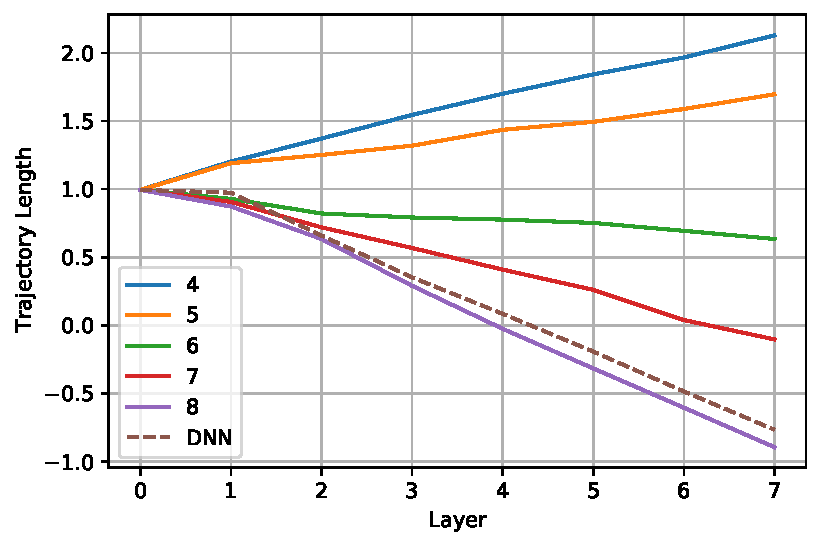
\includegraphics[width=12cm]{latex/figures/TL_untrained.pdf}
    \caption{Logarithmic trajectory length (TL) as a circular trajectory $\boldsymbol{x}(t_i)$ is propagated though QCNs with different number of qubits. The QCNs are defined as in \cref{sec:Vanishing Local Gradients in QCNs}. For comparison, the TL of a DNN with 11 nodes is also shown.}
    \label{fig:TL_untrained}
\end{figure}

\cref{fig:TL_untrained_projection}, accompanying \cref{fig:TL_untrained}, shows the trajectories of selected models and layers, projected onto 2D. The rows correspond to the QCN with four qubits, the QCN with eight qubits, and the DNN, from top to bottom. The columns correspond to the trajectory resulting from the first layer, second layer, third layer and last layer, left to right.   

\begin{figure}[H]
    \centering
    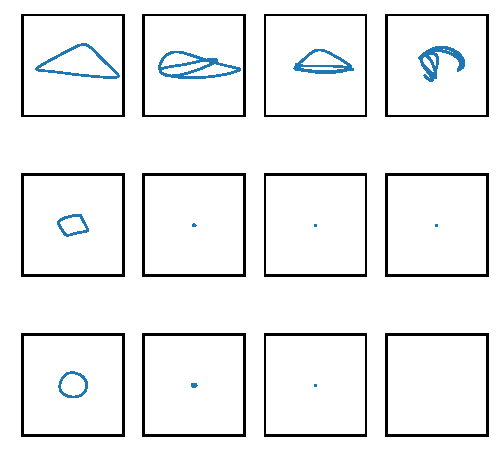
\includegraphics[width=12cm]{latex/figures/TL_untrained_projection.pdf}
    \caption{Trajectory length projected onto 2D for selected models from \cref{fig:TL_untrained}. The rows shows the trajectory length of the four qubits QCN, eight qubit QCN and DNN, from top to bottom. The columns show the trajectory of the first layer, the second layer and last layer, from left to right.}
    \label{fig:TL_untrained_projection}
\end{figure}

%In \cref{fig:TL_untrained}, we see that the untrained DNN exhibits an exponential decrease in trajectory length as it is being transformed by each layer. From \cref{fig:TL_untrained_projection}, we see this manifesting itself as the trajectory concentrating around some mean, progressively more for each layer. This shows that randomly initialized DNNs can tend to compute functions which are not very sensitive to the input, which was shown experimentally by \citet{raghu2017expressive} to be possible in practical settings. 

From \cref{fig:TL_untrained}, we see that the trajectory length of QCNs with 4 and 5 qubits tend to grow exponentially with the number of layers, meaning they are in the exponential growth regime. This growth is however diminishing as the number of qubits increase, and switches over to an exponential decay for 6 qubits and above. For 8 qubits, the decay is similar to that of the DNN with similarly many parameters. Comparing the results to \cref{fig:TL_untrained_projection}, we see how the increasing and decreasing trajectory length manifests themselves. Seen from the top row, the trajectory produced by the 4 qubit QCN tends to become increasingly distorted and complex. This is similar to the behaviour of classical networks seen in \cref{fig:trajectoryLengthExample}, produced by \citet{raghu2017expressive}, and shows that also QCNs can compute functions exponentially complex in the number of layers. In contrast, the trajectory of the 8 qubit QCN and DNN (seen in the next two rows) can be seen to gradually concentrate for each layer, resulting in a function that is very little sensitive to the input.  


%================================================================
\subsection{Trained Models}\label{sec:Trained Models}
%================================================================
\citet{raghu2017expressive} showed that networks that initially don't lie in the exponential growth regime can be pushed there via training. In this subsection, we will train different models by incrementally fitting them to the 2D mixed Gaussian data (see \cref{sec:Mixed Gaussian Data}). The trajectory length will be recalculated for each layer after each increment. The models being investigated here are  QCNs with 6 and 7 qubits, respectively, with each node having the same architecture as in \cref{sec:Vanishing Local Gradients in QCNs}. These will be compared to DNNs with approximately same number of parameters. The models have three hidden layers, with a single node in the output layer. For more information about the models, see \cref{tab:TL models}. All the models are trained using Adam optimizer with the standard hyperparameters and a learning rate of $0.1$. The QCNs are trained for a total of $20$ epochs in increments of $5$. In order to produce a fair comparison, the DNNs will not be trained for the same increments of epochs. Rather, they will be trained until they achieve approximately the same MSE on the training set as the QCNs, for each increment. In this way, we get to compare the expressivity of QCNs and DNNs that fit the data to an equal degree. \cref{fig:TL_trained} shows how the trajectory length changes as the different models presented here are incrementally trained, for each layer. 

\begin{figure}[H]
    \centering
    \begin{subfigure}[t]{0.5\textwidth}
        \centering
        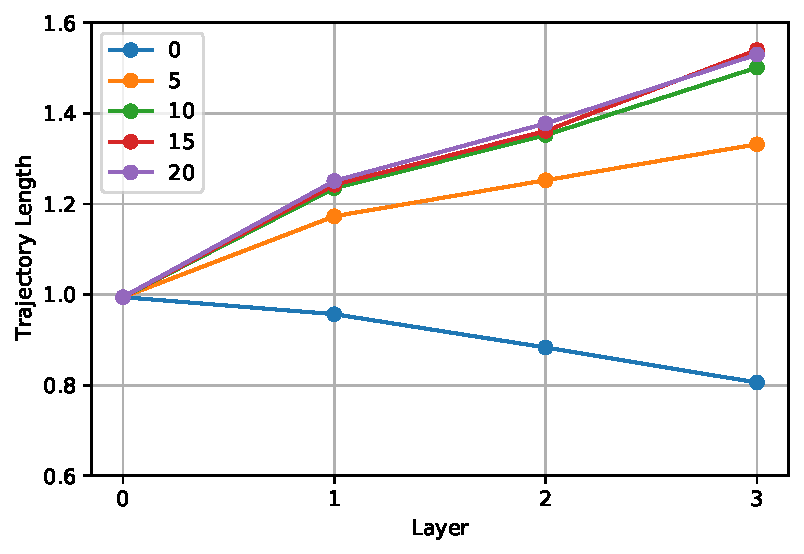
\includegraphics[height=1.9in]{latex/figures/TL_trained_QCN_qubit_6.pdf}
        \caption{QCN, 6 qubits. 228 parameters.}
        \label{fig:TL_trained_A}
        
    \end{subfigure}%
    \hfill 
    \begin{subfigure}[t]{0.5\textwidth}
        \centering
        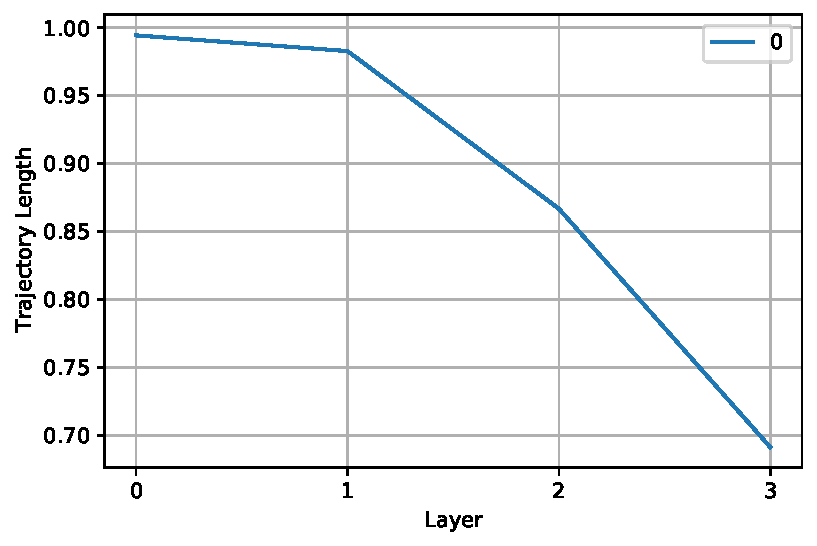
\includegraphics[height=1.9in]{latex/figures/TL_trained_QCN_qubit_7.pdf}
        \caption{QCN, 7 qubits. 308 parameters.}
        \label{fig:TL_trained_B}
    \end{subfigure}
    \vskip\baselineskip
    \begin{subfigure}[t]{0.5\textwidth}
        \centering
        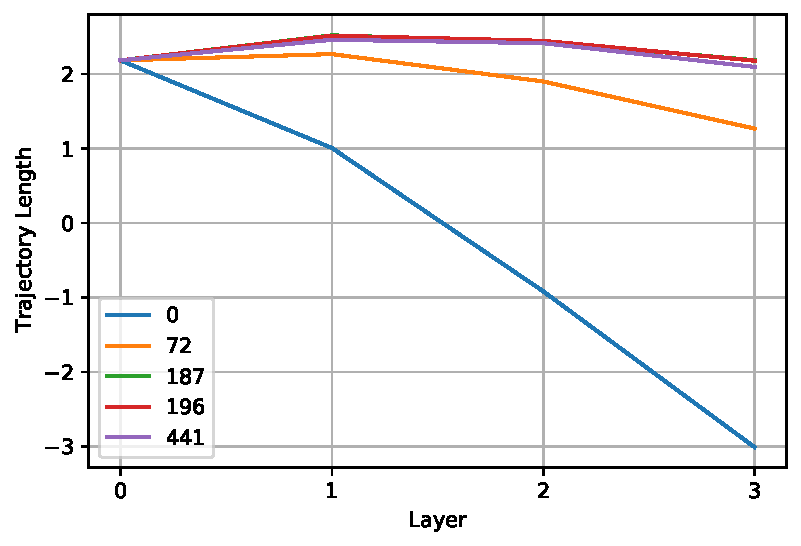
\includegraphics[height=1.9in]{latex/figures/TL_trained_DNN_nodes_9.pdf}
        \caption{DNN, 9 nodes. 217 parameters.}
        \label{fig:TL_trained_C}
        
    \end{subfigure}%
    \hfill 
    \begin{subfigure}[t]{0.5\textwidth}
        \centering
        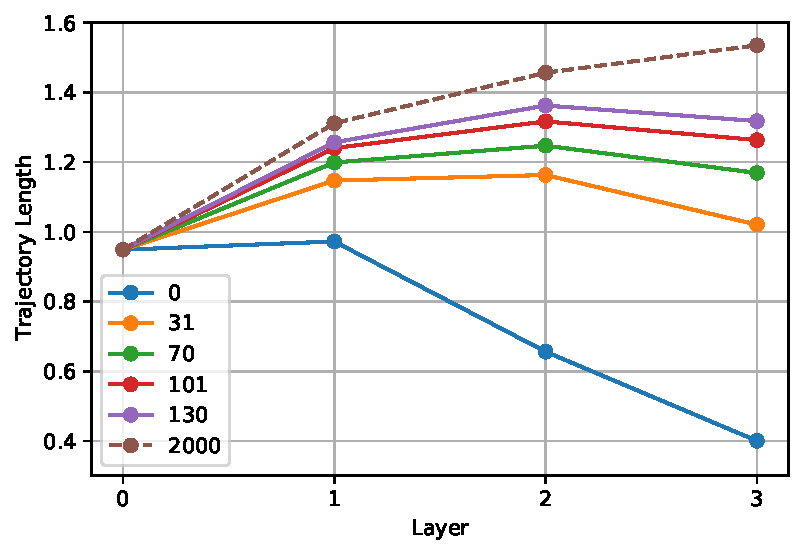
\includegraphics[height=1.9in]{latex/figures/TL_trained_DNN_nodes_11}
        \caption{DNN, 11 nodes. 309 parameters.}
        \label{fig:TL_trained_D}
    \end{subfigure}
    \caption{Logarithmic trajectory length (TL) as a circular trajectory $\boldsymbol{x}(t_i)$ is propagated though QCNs and DNNs defined in \cref{tab:TL models}. The models are gradually fitted for different number of epochs, shown in the legend, and the TL recalculated.}
    \label{fig:TL_trained}
\end{figure}

From \cref{fig:TL_trained}, we see that training the QCNs and DNNs progressively increases the trajectory length of the models. After only $5$ epochs, the trajectory length of the 6 qubit QNC enters the exponential growth regime. This demonstrates that randomly initialized QCNs can be made to produce complex functions through training, even though their outputs initially tend to concentrate around a mean, as shown in \cref{fig:TL_untrained}. The 7-qubit QCN is brought into the exponential growth regime after $10$ epochs, twice the amount required for 6 qubits. 

Moving over to the corresponding DNNs, we see that they fail to enter the same exponential growth regime as the QCNs, even when trained until they fit the data to the same degree. This indicates that QCNs, in this context, may be more expressive than DNNs for the same number of parameters.  

\begin{table}[H]
\centering
\begin{tabular}{|l|l|l|l|l|l|}
\hline
Model &Type & Qubits& Hidden Layers & Nodes &$n_{\theta}$ \\ \hline
A    & QCN & 6 &  3 & 6& 228   \\ \hline
B    & QCN & 7 &  3 & 7& 308 \\ \hline
C    & DNN & NA&  3 & 9& 217  \\ \hline
D    & DNN & NA&  3 & 11& 309  \\ \hline
\end{tabular}
\caption{Hyperparameters of the models in trained on the 2D mixed Gaussian data in \cref{fig:TL_trained}. The DNNs have tanh activation on all layers, including the output layer.} 
\label{tab:TL models}
\end{table}


%================================================================
\subsection{Single Node Expressivity}\label{sec:Single Node Expressivity}
%================================================================
To elucidate the discrepancy of expressivity between QCNs and DNNs, we investigate the functional form of node outputs for QCNs and DNNs. To do this, we use a QCN node (a QNN) with four qubits. It utilizes qubit encoding and two repetitions of the simple ansatz. We prepare data $\boldsymbol{x} = (x, x, x, x)$, and encode it in the usual way. For comparison, we also feed the samples $\boldsymbol{x}$ to a single DNN node with tanh activation. In \cref{fig:activations}, we plot the output the different nodes for different parameter realizations and values of $x$.

\begin{figure}[H]
    \centering
    \begin{subfigure}[t]{0.5\textwidth}
        \centering
        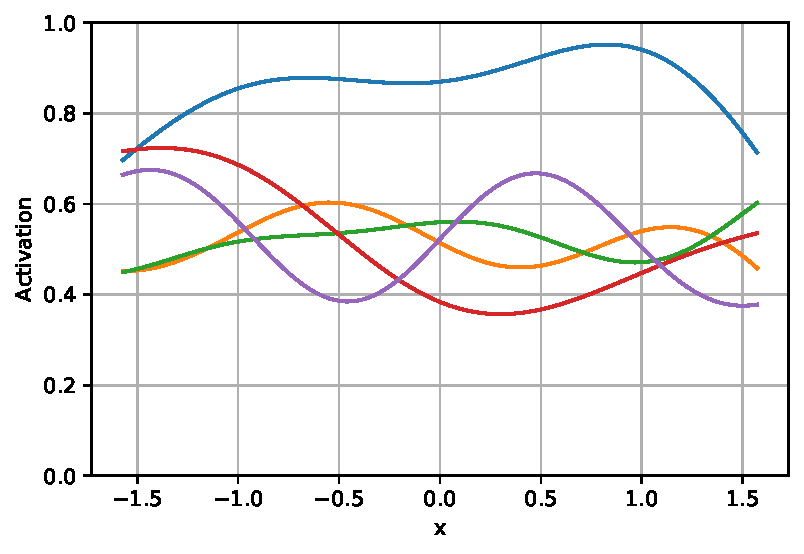
\includegraphics[height=1.9in]{latex/figures/activation_qnn_4.pdf}
        \caption{QCN node with four qubits. It utilizes qubit encoding \cref{fig:qubitencoding} with $R_y$ rotations, and two repetitiaons of the simple ansatz \cref{eq:simple ansatz}.}
        \label{fig:activations tensorial}
    \end{subfigure}%
    \hfill 
    \begin{subfigure}[t]{0.5\textwidth}
        \centering
        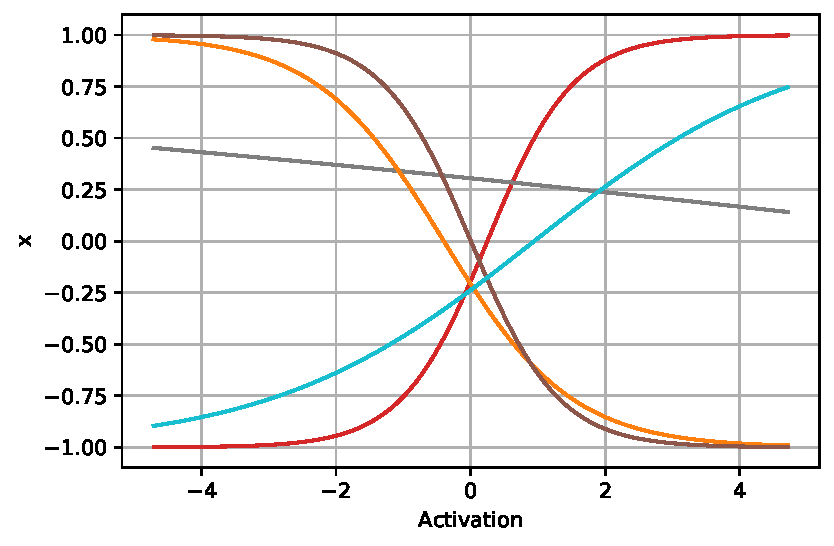
\includegraphics[height=1.9in]{latex/figures/activation_dnn.pdf}
        \caption{DNN node with tanh activation}
        \label{fig:activations DNN}
    \end{subfigure}%
    \caption{Comparison between the functional form of the outputs of a QCN node and a DNN node. The different functions stem from different parameters realizations in the nodes.}
    \label{fig:activations}
\end{figure}

Seen from \cref{fig:activations tensorial}, the QCN node produces a more flexible output, reflecting the polynomial representation of the data in the prepared state \cref{eq:qubit rotation interaction}. \cref{fig:activations DNN} shows that the output of the DNN node is constrained to the functional form of the tanh activation function.   




%================================================================
\subsection{Discussion}\label{sec:Discussion Expressivity}
%================================================================

For higher number of qubits, we saw from \cref{fig:TL_untrained_projection} that the trajectory of untrained QNCs tend to concentrate progressively for each layer they pass through. This is a manifestation of the phenomenon where PQC outputs tends to concentrate around their average value when the number of qubits is increased. Since each node is a QNN, which is a type of PQC, QCN are also subject to this. As the inputs are sequentially transformed by each layer in the QCN, this concentration of the outputs is in fact applied multiple times, causing an exponential decrease of the trajectory length, as seen in \cref{fig:TL_untrained}.

From \cref{fig:TL_trained} we see that training brought the QCNs into the exponential growth regime, increasing the sensitivity of the node outputs with respect to the inputs. In other words, optimizing the QCNs updates the parameters in a way that brings structure to each of the circuits, moving them away from being random circuits. This causes the outputs to no longer concentrate around the mean, which in turn lets the model compute more complex functions. 

Comparing \cref{fig:TL_trained_A} and \cref{fig:TL_trained_B}, we see that the 7-qubit QCN required twice the number of epochs to enter the exponential growth regime compared to the 6-qubit QCN. As discussed in \cref{sec:Vanishing Gradient Phenomenon}, increasing the number of qubits makes the magnitude of the gradient exponentially smaller. Thus, a larger number of epochs, potentially exponentially so, are required to significantly change the parameters such that the nodes no longer resemble random circuits. This might produce a significant overhead for QCNs with a high number of qubits, making them very slow to train to be expressive.  

Looking at \cref{fig:TL_trained_C} and \cref{fig:TL_trained_D}, we see that the corresponding DNNs fail to enter the exponential growth regime, even after training the models for a number of epochs that result in the same MSE as the QCNs. The DNNs approached exponential growth first after more than an order magnitude more epochs. This suggests that QCNs can be trained to be more expressive than DNNs of similar number of parameters. How can we explain this increased expressivity? As discussed in \cref{sec:Single Node Expressivity}, qubit encoding several features results in a representation of exponentially many interactions in the data, which also results in a more flexible output. The different parameter realizations produce very different functional outputs, enabling the QCN to learn unique activations for each node. This is contrast to the outputs of the DNNs, which is very constrained by the Tanh activation function. 

%A possible explanation for this is that the mathematical transformation applied by the QCN is in a way more powerful compared to DNNs. Typically, sufficiently deep PQCs are conjectured to be intractable for classical computers to simulate efficiently \cite{abbas2020power}\cite{lloyd2018quantum}. Stated in \cref{sec:Multiple Qubits}, as the numbers of qubits $n$ increase, the dimensionality of the resulting Hilbert space grows exponentially as $d = 2^n$. It follows that gates applied on this space is mathematically represented as a $d\times d$ matrices, which causes an exponential overhead on classical computers. In this sense, the encoding and unitary transformations of each QCN node constitutes a harder computation than the affine transformation and non-linearity of DNN nodes. Still, even though a computation is harder, it does necessarily result in the computation of a richer, more complicated function. For example, it was shown from \cref{fig:TL_untrained} that the opposite is true for randomly initialized QCNs. However, the increasing trajectory length seen in \cref{fig:TL_trained} suggest that(elaborate). 

%================================================================
\section{Training Models on Mixed Gaussian Data}\label{sec:Training Models}
%================================================================
In this section, we will study the ability of various models to fit one, two and three dimensions mixed Gaussian data. For more details on the data, see \cref{sec:Mixed Gaussian Data}. We will train QNNs, QCN and DNNs with varying complexity and use MSE on the training data to evaluate how good the fit is. This will be done first in the ideal case, with exact calculation of outputs. Then, we will repeat the training using the simulated noise model of the IBM Santiago quantum computer \cite{santiago}. The hyper parameters, such as number of layers, nodes and qubits, are chosen by trial and error such that the results QCNs are relatively small in number of parameters, but still fit the data sufficiently. The QNNs and DNNs are then chosen such that they have similar number of parameters as the QCNs.  For a detailed description of the models trained in this section, see \cref{tab:training models}.

\begin{table}[H]
\centering
\caption{Hyper-parameters of the different models fitted to the one, two, and three dimensional mixed Gaussian data. \emph{Qubits} refer to the number of qubits used in each circuit, and \emph{Reps} refer to the number of repetitions of the simple ansatz \cref{eq:simple ansatz}, and $n_{\theta}$ refers to the number of parameters in the model.} 
\begin{tabular}{|l|l|l|l|l|l|l|l|}
\hline
Model& Type& Data& Qubits& Reps& Layers & Nodes &$n_{\theta}$ \\ \Xhline{3\arrayrulewidth}
A    & QNN & 1D  & 4     & 5&NA     & NA& 20   \\ \hline
B    & QCN & 1D  & 4     & 1&2      & 4& 20 \\ \hline
C    & QCN & 1D  & 4     & 2&2      & 4& 40  \\ \hline
D    & DNN & 1D  & NA    & NA&2      & 13& 40  \\ \Xhline{3\arrayrulewidth}
E    & QNN & 2D  & 4     & 10&NA     & NA& 40  \\ \hline
F    & QCN & 2D  & 4     & 1&3      & 4& 40  \\ \hline
G    & QCN & 2D  & 4     & 2&3      & 4& 80  \\ \hline
H    & DNN & 2D  & NA    & NA&3      & 7& 85  \\ \Xhline{3\arrayrulewidth}
I    & QNN & 3D  & 5     & 11&NA     & NA& 55  \\ \hline
J    & QCN & 3D  & 5     & 1&3      & 5& 55  \\ \hline
K    & QCN & 3D  & 5     & 2&3      & 5& 110  \\ \hline
L    & DNN & 3D  & NA    & NA&3      & 8& 113  \\ \hline
\end{tabular}

\label{tab:training models}
\end{table}

For the QNNs trained in this section, we will utilize RZZ encoding \cref{fig:Rzzencoding} together with latent qubits \cref{fig:latent qubits} in an effort to increase the flexibility of the model. From \cref{sec:RZZencoding}, we know that the circuit depth of this encoding scales as $\mathcal{O}(p^2)$, where $p$ is the number of features. To get a constant depth across the 1D, 2D and 3D Gaussian data, we will repeat features until all the data sets have the same number of features: For the 1D data, we repeat the one feature three times: $(x_1) \rightarrow (x_1, x_2, x_3)$. For the 2D data, we repeat the first feature once: $(x_1, x_2) \rightarrow (x_1, x_2, x_1)$. The 3D data is left unchanged, since it already has three features. In this way, RZZ encoding prepares similarly complicated encoding for all data sets.


%================================================================
\subsection{Ideal Simulation}\label{sec:Ideal Simulation}
%================================================================
\cref{fig:trained ideal} shows the MSE during training of the models defined in \cref{tab:training models} on the one, two and three dimensional mixed Gaussian data. All models are trained for 100 epochs, using Adam optimizer and ideal simulation. In order to produce a more significant result, each model is randomly initialized ten times and trained separately. The resulting MSE for each model is then averaged over the 10 runs and plotted with fill corresponding to one standard deviation. In this way, we get to see the average model behaviour during training and how it varies between different runs. \cref{tab:training models mse} shows the final MSE after 100 epochs for the various models. In addition, the final MSE after $10^4$ epochs is included for the DNNs.   

\begin{figure}[H]
    \centering
    \begin{subfigure}[t]{0.45\textwidth}
        \centering
        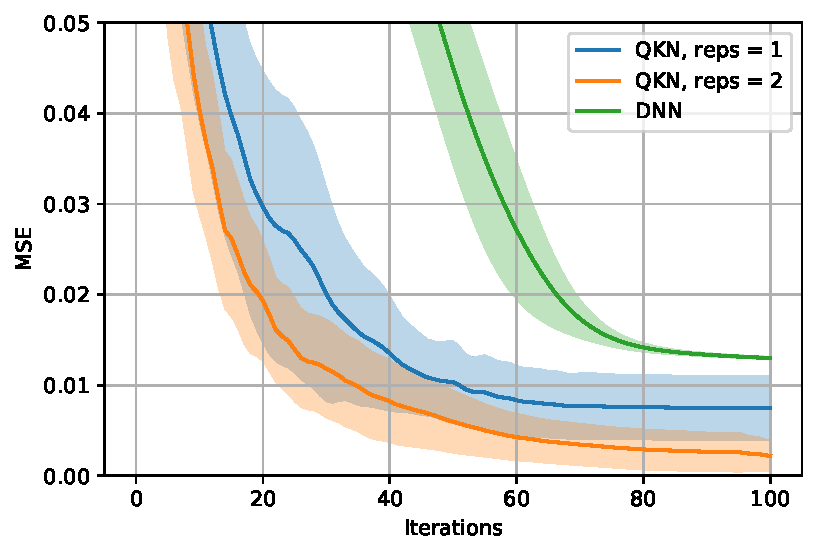
\includegraphics[height=1.9in]{latex/figures/1D_gaussian_data_fit.pdf}
        \caption{MSE of models trained on 1D mixed Gaussian data.}
        
    \end{subfigure}%
    \hfill 
    \begin{subfigure}[t]{0.45\textwidth}
        \centering
        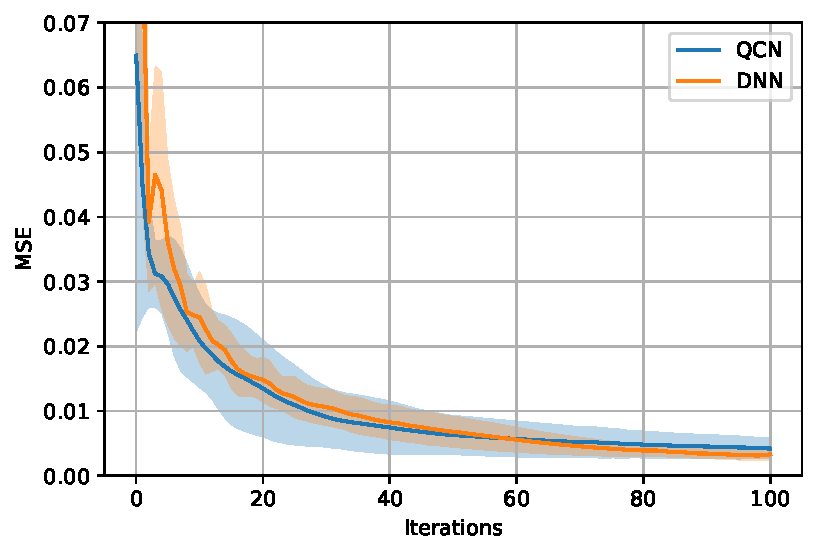
\includegraphics[height=1.9in]{latex/figures/2D_gaussian_data_fit.pdf}
        \caption{MSE of models trained on 2D mixed Gaussian data.}
    \end{subfigure}
    \vskip\baselineskip
    \begin{subfigure}[t]{0.45\textwidth}
        \centering
        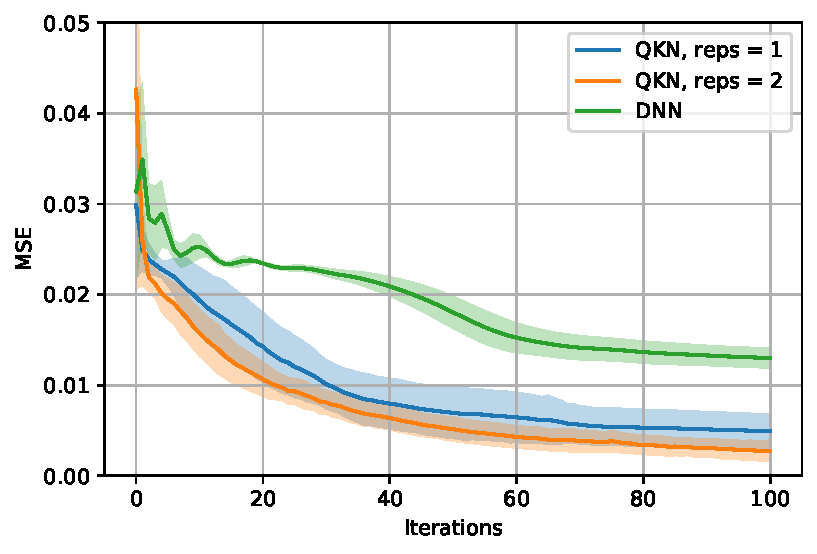
\includegraphics[height=1.9in]{latex/figures/3D_gaussian_data_fit.pdf}
        \caption{MSE of models trained on 3D mixed Gaussian data.}
        
    \end{subfigure}%
    \caption{MSE during training of the models defined in \cref{tab:training models}, trained on the mixed Gaussian data (see \cref{sec:Mixed Gaussian Data} for details on the data). The QNNs and QCNs are trained using ideal simulations.}
    \label{fig:trained ideal}
\end{figure}

\begin{table}[H]
\centering
\caption{Final MSE after training of the models detailed in \cref{tab:training models}, using ideal simulation These results accompany the training shown in \cref{fig:trained ideal}. The lowest MSE after 100 epochs is highlighted.}
\begin{tabular}{|l|l|l|l|l|}
\hline
Model& Type& Data& MSE, $10^{2}$ Epochs& MSE, $10^{4}$ Epochs \\ \hline
A    & QNN & 1D  &  $4.6\times 10^{-2}$  & NA   \\ \hline
B    & QCN & 1D  & $5.9\times 10^{-3}$  & NA \\ \hline
C    & QCN & 1D  & $\boldsymbol{8.0\times 10^{-4}}$  & NA  \\ \hline
D    & DNN & 1D  & $9.2\times 10^{-3}$ & $2.2\times 10^{-4}$  \\ \Xhline{2\arrayrulewidth}
E    & QNN & 2D  &  $3.6\times 10^{-2}$ & NA  \\ \hline
F    & QCN & 2D  &  $1.8\times 10^{-2}$ & NA  \\ \hline
G    & QCN & 2D  &  $\boldsymbol{4.3\times 10^{-3}}$ & NA  \\ \hline
H    & DNN & 2D  &  $4.5\times10^{-2}$ & $4.3\times10^{-3}$\\ 
\Xhline{2\arrayrulewidth}
I    & QNN & 3D  &  $2.0\times 10^{-2}$& NA  \\ \hline
J    & QCN & 3D  &  $4.9\times 10^{-3}$ & NA  \\ \hline
K    & QCN & 3D  &  $\boldsymbol{2.8\times10^{-3}}$  & NA  \\ \hline
L    & DNN & 3D  &  $1.2\times10^{-2}$  & $1.8\times10^{-3}$  \\ \hline
\end{tabular}
 
\label{tab:training models mse}
\end{table}

From \cref{fig:trained ideal}, we see that the QCNs minimize the MSE quicker than both the QNNs and DNNs on the mixed Gaussian data, for any number of dimensions. The QCNs with the two ansatz repetitons also trained faster than those with just one. Further, we see that QNNs perform overall worst among the models. After initially fast optimization, the models quickly flatten out at a relatively high MSE, struggling to obtain a good fit. From \cref{tab:training models}, we see that the DNNs obtains the lowest MSE among all models when trained until saturation, after $10^4$ epochs.


%================================================================
\subsection{Noisy Simulation}\label{sec:Noisy Simulation}
%================================================================
In this section, we investigate how QNNs and QCNs behave when trained on the Gaussian data using simulated quantum hardware. We do this by repeating the training of the models of last subsection using a simulation of the Santiago quantum computer \cite{santiago}. We exclude, however, the training on the 3D mixed Gaussian due to the huge computational burden of simulating real hardware. The resulting MSE during training can be seen in \cref{fig:trained noisy}. Each model was trained for 100 epochs, using 1024 shots to estimate the output of each circuit. \cref{tab:training models mse noisy} shows the final MSE after 100 epochs for the QNNs and QCNs, trained on simulated hardware. As earlier, the resulting MSE after 100 and $10^{4}$ epochs is also included for the DNNs.


\begin{figure}[H]
    \centering
    \begin{subfigure}[t]{0.45\textwidth}
        \centering
        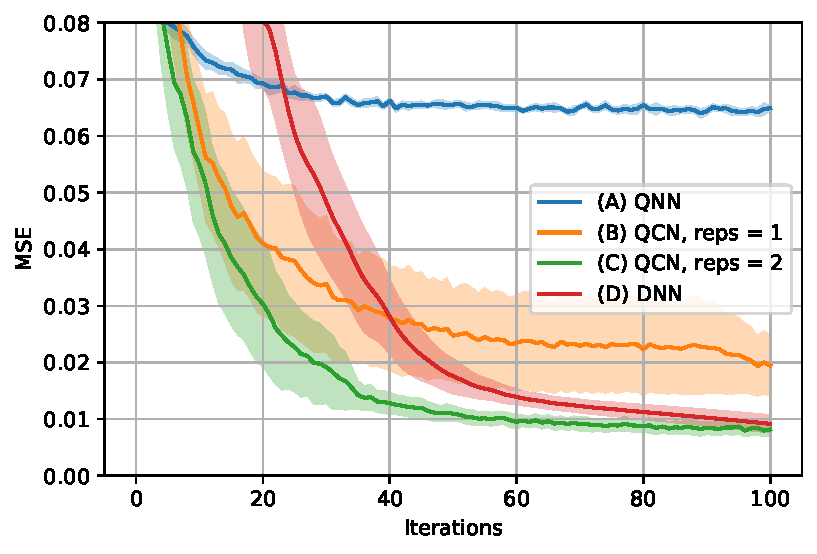
\includegraphics[height=1.9in]{latex/figures/1D_gaussian_data_fit_noisy.pdf}
        \caption{MSE of models trained on 1D mixed Gaussian data.}
        
    \end{subfigure}%
    \hfill 
    \begin{subfigure}[t]{0.45\textwidth}
        \centering
        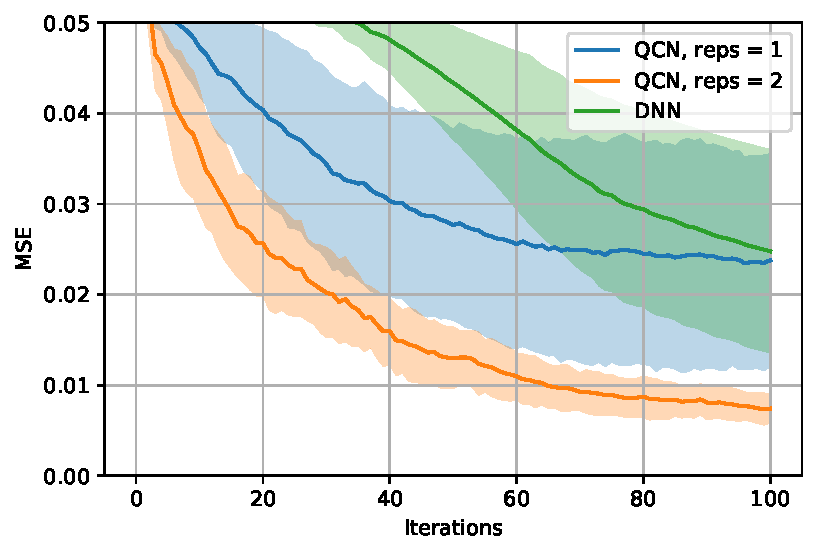
\includegraphics[height=1.9in]{latex/figures/2D_gaussian_data_fit_noisy.pdf}
        \caption{MSE of models trained on 2D mixed Gaussian data.}
    \end{subfigure}
    \caption{MSE during training of the models defined in \cref{tab:training models}, trained on the mixed Gaussian data, excluding the 3D data (see \cref{sec:Mixed Gaussian Data} for details on the data). The QNNs and QCNs are trained using noisy simulation of the Santiago quantum computer \cite{santiago}, using the methods of \cref{sec:Noisy Simulation}.}
    \label{fig:trained noisy}
\end{figure}


\begin{table}[H]
\centering
\caption{Final MSE after training the models detailed in \cref{tab:training models}, using noisy simulation of the Santiago quantum computer \cite{santiago}. See \cref{sec:Noisy Simulation} for details. These results accompany the training shown in \cref{fig:trained noisy}.} 
\begin{tabular}{|l|l|l|l|l|}
\hline
Model& Type& Data& MSE, $10^{2}$ Epochs& MSE, $10^{4}$ Epochs \\ \hline
A    & QNN & 1D  & $6.6 \times 10^{-2}$   & NA   \\ \hline
B    & QCN & 1D  & $2.0\times 10^{-2}$  & NA \\ \hline
C    & QCN & 1D  & $\boldsymbol{8.2\times 10^{-3}}$  & NA  \\ \hline
D    & DNN & 1D  & $1.1\times 10^{-2}$ & $3.1\times 10^{-2}$  \\ \Xhline{2\arrayrulewidth}
E    & QNN & 2D  &  $4.0 \times 10^{-2}$                  & NA  \\ \hline
F    & QCN & 2D  &  $2.4\times 10^{-2}$ & NA  \\ \hline
G    & QCN & 2D  &  $\boldsymbol{7.4\times 10^{-3}}$ & NA  \\ \hline
H    & DNN & 2D  &  $2.5\times10^{-2}$ & $1.6\times10^{-3}$\\\hline
\end{tabular}

\label{tab:training models mse noisy}
\end{table}

Comparing \cref{fig:trained noisy} and \cref{fig:trained ideal}, we see that the QNNs and QCNs trained on noisy hardware train slower and obtain a overall higher final MSE after 100 epochs, compared to the ideal simulation. 


%================================================================
\subsection{Discussion}\label{sec:Training Discussion}
%================================================================
In \cref{sec:Vanishing Gradient Phenomenon} and \cref{sec:Investigating the Loss Landscape}, it was suggested that QCNs of few qubits and layers would train faster than DNNs with similar number of parameters, due to their relatively larger gradient and more uniform EFIM spectrum. As we see from \cref{fig:trained ideal}, this is indeed the case when training on the mixed Gaussian data using exact and noiseless simulation.
Further, we see that the QCNs with two ansatz repetitions show faster training and less variance than those with only one repetition. This shows that QCNs can be made more flexible by adding additional complexity to each node in the form of additional repetitions. 

In \cref{sec:Expressivity}, it was suggested that QCNs are more expressive and flexible than DNNs with similar number of parameters. Looking at \cref{tab:training models mse}, we see that the final MSE obtained by the QCNs with two repetitions is within the same order of magnitude as the final MSE obtained by the DNNs. This is despite the fact that the QCNs were only trained for 100 epochs, while the DNNs where allowed to train for $10^4$ epochs (basically until saturation, i.e. the lowest possible MSE for that particular model). In light of this, it is not unlikely that the QCNs would eventually reach a lower MSE than the DNNs if given the opportunity to train for more epochs. This suggests that it is possible for QCNs to fit complicated data more easily than DNNs, and hence are more flexible. However, this is speculative, as we are unable to train the QCNs much further due to limited computational resources.    

We see in \cref{fig:trained ideal} that they struggle to obtain a good fit on the mixed Gaussian data, even though they have a similar number of parameters as the QCNs with one ansatz repetition. This shows that RZZ encoding combined with multiple repetitions of the simple ansatz is insufficient for fitting this data. As explained in \cref{sec:FeedForward}, our QNNs perform a mostly unitary (and thus linear) transformation of the input, except at the stage of encoding and measurement. This results in a perhaps too constrained model, which might explain the QNNs' inability to fit the data. QCNs, on the other hand, incorporate multiple non-linearities for each layer as a result of measurements done to estimate the output of each node, as explained in \cref{sec:Quantum Circuit Network}. As with DNNs, this is likely the key to their greater flexibility, as it enables them to compute a larger family of functions. 

Moving over to the training using the simulated noisy hardware, we see from \cref{fig:trained noisy} that the QNN and QCN models performed overall worse than in the ideal case. This is not surprising, since the simulation of real hardware and the low number of 1024 shots cause a significant amount of noise to be added to the outputs of the QNNs and QCNs. The slowdown of the training is likely a due to noise being added to the calculation of the gradient. This causes it to misalign with the direction of steepest descent, as discussed in \cref{sec:BarrenPlateus}, and which results in the optimization slowing down. However, the QCNs with two ansatz repetitions still obtained a lower MSE than the DNNs after 100 epochs, even in using the noisy simulation. This shows that QCNs have the ability to outperform DNNs on some data sets, even on noisy quantum hardware with few shots. 


%================================================================
\section{Real-World Data}\label{sec:Real Data}
%================================================================
In this section, we compare the performance QCNs and DNNs by performing regression on the Boston Housing data \cite{boston} and classification on the Breast Cancer Wisconsin data \cite{cancer}. To reduce the computational burden of training the models, both data sets are feature reduced to four features using principal component analysis (PCA). See \cref{sec:Appendix B} for more information about the data sets. To uncover how well the models generalize, we will test their performance on independent training and test sets using MSE as a metric. For the Breast Cancer data, we will also investigate the training and test accuracy \cref{eq:accuracy}. 
%The models will be benchmarked using MSE on both the the training set and an independent test set, as explained in \cref{sec:Generalizability}. This is done to uncover how the models generalize to unseen data. For the Breast Cancer Wisconsin data, we will also investigate the training and test accuracy \cref{eq:accuracy} of the models.

The QCNs models are chosen to have four qubits in each circuit, and only two layers. This is done to obtain a model that has a large gradient due to low number of qubits, as discussed in \cref{sec:Vanishing Gradient Phenomenon Discussion}, and are thus easy to train. The DNNs are chosen such that the number of parameters approximately match that of the QCNs. The hyperparameters of the various models are listed in \cref{tab:training models PCA}.

%For both the feature reduced and full data set, we will split the data sets into independent training and test sets at random, each with $N=100$ samples. The targets of the Boston Housing data is min-max scaled to $y \in [0,1]$, while the discrete targets of the Breast Cancer data are already $y \in \{0,1\}$.

%To reduce the number of features, the training and test data sets are each reduced to four features using PCA and scaled appropriately depending on the model, as explained in \cref{sec:Pre-processing Input}. The hyperparameters of the various models trained on the feature reduced data is listed in \cref{tab:training models PCA}.



\begin{table}[H]
\centering
\caption{Hyperparameters of the various models fitted to the feature reduced Boston Housing data and Breast Cancer data.} 
\begin{tabular}{|l|l|l|l|l|l|l|l|}
\hline
Model& Type& Data& Qubits& Reps& Layers & Nodes &$n_{\theta}$ \\ \hline
A    & QCN & Boston Housing Data  & 4     & 2  &2     & 4& 40   \\ \hline
B    & DNN & Boston Housing Data  & NA    & NA &2     & 6& 37 \\ \Xhline{2\arrayrulewidth}
C    & QCN & Breast Cancer        & 4     & 2  &2     & 4& 40  \\ \hline
D    & DNN & Breast Cancer        & NA    & NA &2     & 6& 37  \\ \hline
\end{tabular}

\label{tab:training models PCA}
\end{table}

The models defined in \cref{tab:training models PCA} are trained for 100 epochs, ten times each for different random initializations of parameters.  In \cref{tab:results PCA}, we see the average minimum training and test MSE for each model obtained during training. In addition, the final average training and test accuracy is included for the models trained on the Breast Cancer data. We see that the training MSE is strictly lower than the test MSE, i.e., both the QCN and DNN does not perform as good on the test set as on the training set. As explained in \cref{sec:Generalizability}, we know that since the models are optimized with respect to the training set, its performance on the independent test set will always be worse. Comparing the models trained on the Boston Housing data, we see that the QCN has a lower test MSE than the DNN, meaning it generalizes better to unseen data. The same is however not true for the Breast Cancer data, where the QCN obtained almost twice the test MSE compared to the DNN. This indicates that the QCN is struggling to produce the correct labels $y^{(i)} \in \{0, 1\}$ which are the targets of the Breast Cancer data. Hence, both the train and test accuracies are lower for the QCN compared to the DNN. 
\begin{table}[H]
\centering
\caption{Hyper-parameters of the different models fitted to the Boston Housing data and Breast Cancer data.} 
\begin{tabular}{|l|l|l|l|l|}
\hline
Model& Type& Data& MSE (train/test)& Accuracy (train/test) \\ \hline
A    & QCN & BHD  & 0.004/$\boldsymbol{0.043}$ & NA    \\ \hline
B    & DNN & BHD  & 0.006/0.052                & NA  \\ 
\Xhline{2\arrayrulewidth}
C    & QCN & Breast Cancer        & 0.028/0.058                & 0.989/0.947    \\ \hline
D    & DNN & Breast Cancer        & 0.001/\boldsymbol{$0.032$} & 1.000/\boldsymbol{$0.965$}  \\ \hline
\end{tabular}

\label{tab:results PCA}
\end{table}


Since these data originate from real world experiments, they are noisy and don't represent a deterministic relationship $y = f(\boldsymbol{x})$ between the target and the features. This is in contrast to the the mixed Gaussian data sets studied earlier, and should provide a more practical benchmark of the methods.